% SPDX-License-Identifier: CC-BY-SA-4.0
%
% Copyright (c) 2020 Philipp Le
%
% Except where otherwise noted, this work is licensed under a
% Creative Commons Attribution-ShareAlike 4.0 License.
%
% Please find the full copy of the licence at:
% https://creativecommons.org/licenses/by-sa/4.0/legalcode

\chapter{Spread Spectrum and Multiple Access}

\begin{refsection}
	
The electromagnetic spectrum is a sparse resource. It must be used as efficient as possible because it is shared with numerous users and applications. However, modern digital communication systems use spread spectrum technologies that occupy a relatively wide frequency band

The purpose of spread spectrum is amongst others:
\begin{itemize}
	\item Immunity against noise and disturbances
	\item Encryption and confidentiality of the communication
	\item Plausible deniability that the communication had ever taken place
	\item Coexistence with other services (multiple access)
\end{itemize}

Especially, the multiple access is an important reason for employing spread spectrum technologies. In modern communication systems, the resource \emph{frequency} is not only allocated to a single user. For example, \ac{LTE} allows many users to access the service with high data rates and low latency. The resource \emph{frequency} must be shared. Efficient medium access relies on spread spectrum to achieve this.

\section{Spread Spectrum}

In the modulation techniques considered so far, are \emph{plain} or \emph{non-spread spectrum}. For the definition of spread spectrum signals, the symbol duration and the transmission bandwidth is investigated.
\begin{itemize}
	\item The signal duration is the amount of time required to convey an information. In digital communication system, an information is a symbol modulated onto a carrier. The signal duration is the symbol period $T_{sym}$.
	\item The signal bandwidth $\Delta f_{sym}$ is the minimum bandwidth required by the receiver to receive the signal. In the case of modulation, it is the \emph{transmission bandwidth}.
\end{itemize}
In the \ac{ASK}, \ac{PSK} and \ac{QAM} modulation of Chapter 5, the signal duration and the bandwidth are inversely proportional.
\begin{equation}
	\Delta f_{sym} = \frac{1}{T_{sym}}
\end{equation}

The product of the bandwidth and the duration -- the \index{time-bandwidth product} \textbf{time-bandwidth product} -- is constantly $1$.\footnote{This is the ideal case. For real implementations, the constant may differ from $1$ depending on the modulation technique. However, it will be close to $1$.}
\begin{equation}
	T_{sym} \cdot \Delta f_{sym} = 1
\end{equation}

\paragraph{Time-Bandwidth Product.}

The time-bandwidth product is used for the definition of spread spectrum:
\begin{definition}{Spread spectrum}
	The time-bandwidth product of \index{spread spectrum} \textbf{spread spectrum} signals is significantly greater than $1$.
	\begin{equation}
		T_{sym} \cdot \Delta f_{sym} \gg 1
	\end{equation}
\end{definition}

Typically, this means that the bandwidth $\Delta f_{sym}$ is increased while the symbol duration and thereby the symbol rate is kept constant.
\begin{itemize}
	\item The symbol sequence (time-bandwidth product of $1$) is altered in a way which distributes the signal power over a wider frequency band. This process is called \index{spreading} \textbf{spreading}.
	\item The inverse process is \index{despreading} \textbf{despreading}. The original symbol sequence is reconstructed from the wide-band spread spectrum signal.
\end{itemize}

\begin{figure}[H]
	\centering
	\begin{tikzpicture}
		\begin{axis}[
			height={0.15\textheight},
			width=0.8\linewidth,
			scale only axis,
			xlabel={$\omega$},
			ylabel={$|\mathrm{S}_{XX}|$},
			%grid style={line width=.6pt, color=lightgray},
			%grid=both,
			grid=none,
			legend pos=north east,
			axis y line=middle,
			axis x line=middle,
			every axis x label/.style={
				at={(ticklabel* cs:1.05)},
				anchor=north,
			},
			every axis y label/.style={
				at={(ticklabel* cs:1.05)},
				anchor=east,
			},
			xmin=0,
			xmax=10.5,
			ymin=0,
			ymax=1.2,
			xtick={0},
			xticklabels={0},
			ytick={0},
			axis x discontinuity=parallel,
		]
			\addplot[blue, smooth] coordinates {(4.6,0) (4.7,0.02) (4.8,0.2) (4.9,0.71) (5,1) (5.1,0.71) (5.2,0.2) (5.3,0.02) (5.4,0)};
			\addlegendentry{Narrow-band signal};
			\addplot[red, smooth] coordinates {(2,0) (2.5,0.01) (3,0.05) (5,0.05) (7,0.05) (7.5,0.01) (8,0)};
			\addlegendentry{Spread spectrum signal};
		\end{axis}
	\end{tikzpicture}
	\caption[PSD of a narrow-band and spread spectrum signal]{\acs{PSD} of a narrow-band and spread spectrum signal. Both signals carry the same information and have the equal power. The narrow-band signal concentrates the whole signal power in a narrow frequency band. In contrast, the spread spectrum signal distributes the signal power over a wide frequency band.}
\end{figure}

\paragraph{Noise-like Signal.}

The signal power remains constant while the signal is spread.
\begin{itemize}
	\item The \ac{PSD} is reduced.
	\item But, the \ac{PSD} is integrated over a wider frequency range.
	\item The overall power remains constant.
\end{itemize}

The \ac{PSD} of the spread spectrum signal is flat in approximation.
\begin{itemize}
	\item The flat \ac{PSD} resembles the \ac{PSD} of noise.
	\item Spread spectrum signal are therefore \emph{noise-like}.
\end{itemize}

A third party who has no knowledge of neither the existence of the spread spectrum signal nor the technology used cannot detect the signal.
\begin{itemize}
	\item The spread spectrum signal looks like noise or a wide-band disturbance from the view of the receiver which does not participate in the communication.
	\item This circumstance can be used to conceal the existence of the signal (plausible deniability of its existence).
\end{itemize}

\paragraph{Despreading.}

\index{despreading} Despreading reconstructs the symbols -- and thereby the data -- from the spread spectrum signal.
\begin{itemize}
	\item The spreading is reversed.
	\item The symbols (time-bandwidth product of $1$) are reconstructed. This can be seen like re-concentrating the spread signal power in a narrow-band symbol sequence.
	\item The disturbances which are uncorrelated to the spread spectrum signal are converted into the wide-band noise with a low \ac{PSD}.
	\begin{itemize}
		\item The wide-band noise floor (like thermal noise or quantization noise) remains wide-band.
		\item Strong but narrow-band disturbing signals (like other users of the electromagnetic spectrum) are spread to low-\acs{PSD} wide-band noise during the despreading. The \ac{SNR} is increased by spreading the signal power of the disturbance.
	\end{itemize}
\end{itemize}

\todo{Despreading in frequency-domain, suppression of noise and disturbances}

\subsection{Direct-Sequence Spread Spectrum}

\todo{pseudorandom number}

\todo{Processing Gain}

\subsection{Frequency-Hopping Spread Spectrum}

\subsection{Time-Hopping Spread Spectrum}

\subsection{Symbol Reconstruction}

\todo{Reception under noise}

\todo{Cross-correlation}

\section{Multi-carrier Modulation}

\todo{OFDM}

\section{Multiple Access}

\todo{Multiplexing}

\todo{Sharing Resources}

\subsection{Space-Division Multiple Access}

\subsection{Time-Division Multiple Access}

\subsection{Frequency-Division Multiple Access}

\subsection{Code-Division Multiple Access}

\subsection{Orthogonal Frequency-Division Multiple Access}

\section{Orthogonal Codes}

\nocite{ipatov2005}

\phantomsection
\addcontentsline{toc}{section}{References}
\printbibliography[heading=subbibliography]
\end{refsection}

